\documentclass[12pt, a4paper] {ncc}
\usepackage[utf8] {inputenc}
\usepackage[T2A]{fontenc}
\usepackage[english, russian] {babel}
\usepackage[usenames,dvipsnames]{xcolor}
\usepackage{listings,a4wide,longtable,amsmath,amsfonts,graphicx}
\usepackage{indentfirst}
\usepackage{bytefield}
\usepackage{multirow}
\usepackage{float}
\usepackage{caption}
\usepackage{subcaption}
\captionsetup{compatibility=false}
\usepackage{tabularx}
\usepackage{pdfpages}

\usepackage[left=2cm,right=2cm,top=2cm,bottom=2cm,bindingoffset=0cm]{geometry}

\begin{document}
\setcounter{figure}{0}
\frenchspacing
\pagestyle{empty}
\begin{center}
                            Университет ИТМО    \\
					Мегафакультет компьютерных технологий и управления \\ 
					Факультет программной инженерии и компьютерной техники \\
                        Кафедра вычислительной техники

\vspace{\stretch{2}}
                Системы ввода/вывода и периферийные устройства
\end{center}
\vspace{\stretch{2}}
\begin{center}
				Лабораторная работа № 1 \\
			{\it «Проектирование вычислительной системы с блоками
				  анализа и формирования цифровых периодических сигналов»}\\
					Вариант 8
\end{center}
\vspace{\stretch{3}}
\begin{flushright}
                                    Студенты:\\
                                    {\it Куклина М.Д.}\\
                                    {\it Кириллова А.А.}\\
                                    Преподаватель: \\
                                    {\it Быковский С.В.}
\end{flushright}
\vspace{\stretch{4}}
\begin{center}
                             Санкт-Петербург, 2017
\end{center}
\newpage

%\tableofcontent

\section{Задание}
    Разработать модель вычислительной системы на языке SystemC. Модель представляет
собой ВС с блоком формаирования цифрового сигнала (Ouput Compare). Необходимо с
помощью этой ВС сгенерировать последовательность 110 (двоичное число, 3 бита) с
заданной длительностью каждого символа. Длительность каждого символа задаётся с
помощью аргумента командной строки при вызове модели на исполнение.

\section{Блок-схема огранизации ПО процессора}

	На <<процессоре>> выполнятся алгоритм по генерации последовательности $011$.
	При длине от $2$ таков это получается путём запуска двух таймеров с периодом в заданную длительность
	и тройную длительность соответственно и переключением их в блоке {\it Output Compare}
	по высчитанному на основе длительности переключения таймеров в блоке {\it OC} времени. 
	При длина сигнала в $1$ такт {\it OC} просто переводится в один из его режимов.

	Рис. 4.

\section{Временные диаграммы обмена данными по шине между блоками схемы}
Диаграмма чтения.
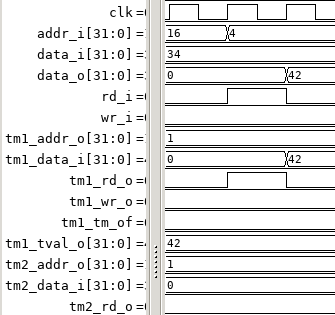
\includegraphics[scale=0.7]{./diagram_read.png}

Диаграмма записи.
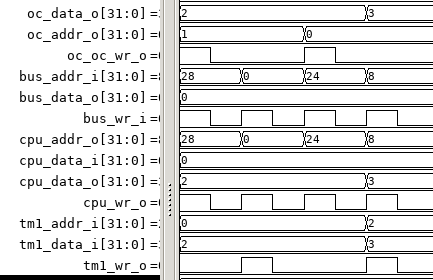
\includegraphics[scale=0.7]{./diagram_write.png}

\section{Временные диаграммы изменения сигналов выхода {\it OutputComapre}}

\begin{figure}[h!]
    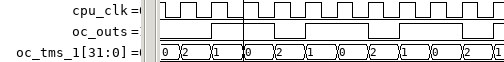
\includegraphics[scale=0.8]{./d1.png}
	\caption{Диаграмма для длительности $ = 1$.}
\end{figure}

\begin{figure}[h!]
    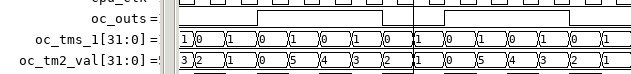
\includegraphics[scale=0.8]{./d2.png}
	\caption{Диаграмма для длительности $ = 2$.}
\end{figure}

\begin{figure}[h!]
    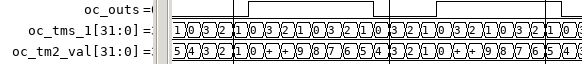
\includegraphics[scale=0.8]{./d4.png}
	\caption{Диаграмма для длительности $ = 4$.}
\end{figure}

\newpage
\begin{figure}[h!]
    
\includegraphics[scale=0.3]{./flowchart.png}
	\caption{Блок-схема ПО процессора}
	\label{flowchart}
\end{figure}

\clearpage

\end{document}
